\chapter{Background} \label{chap:background}
Generally, the first part of every machine learning project is to choosing the algorithm to tackle the problem in hand. As I stated in the proposal of this project, I choose to apply specific machine learning algorithms called Artificial Neural Networks (ANNs) to tackle the classification challenge of detecting pneumonia in X-ray images. The first part of this chapter I would like to provide some information to justify that decision. 

The objective of the algorithm in this report is to classify X-ray images with or without pneumonia. Classification is a task of determining what is the defined class of an example given its data associated with it. In our case, we defined our classes for prediction to the person in the example image having pneumonia or not. In order to achieve that goal, machine learning algorithm must produce a function that outputs the class within defined finite possible classes such as \(f:\mathbb{R}^n \rightarrow \{1, \ldots, k\ \}\) which in this case k is equal to 2. In essence all machine learning algorithms will map input representation of the data \textbf{\textit{x}} to prediction output $\hat{y}=f(x)$. The only difference is how each algorithm is representing the data distribution with a model $f$. Which consequently leads to the question of which algorithm is the best algorithm for machine learning or which algorithm to choose to find the best model representation. According to \textbf{no free lunch theorem}~\cite{nofreelunch} there is no such algorithm exist that will consistently achieve low error rate averaged over all possible distributions. In other words, no model is universally any better than any other machine learning model. Luckily, the objective in this project is not to find the universally best algorithm but rather to find the algorithm that will find the best representation for the data distribution of healthy and pneumonia X-ray images. 
Historically, traditional machine learning algorithms often performed poorly on tasks such as computer vision, detecting objects or speech recognition. Part of the reason is these task usually involve high-dimensional data. Because many traditional machine learning algorithms assume that any unseen data point should be similar to nearest training point, generalization in high-dimensional data such as image classification also suffers due to the fact that data points in these space are spread out and the notion of similarity weakens. Effect of this high-dimensionality also known as \emph{curse of dimensionality}.
Because of the weakness described earlier, Artificial Neural Networks emerges as a clear choice for image classification and object detection task which became evident with the performance of AlexNet~\cite{Alexnet}, VGGNet~\cite{vggnet} and ResNet~\cite{resnet} in the ILSVRC~\cite{imagenet}.  


\section{Building Blocks of ANN} \label{sec:bbann}
The idea of Artificial Neural Networks inspired by the neural cells of the human brain. Earliest known research for ANNs dates back to 1943 as a multidisciplinary work of phycology and mathematics by Warren McCulloch and Walter Pitts~\cite{firstann}. Their work covered how computational logic could model complex neural cells activities. However, first development that reshaped the way for current generally accepted practices of ANNs was the work of Frank Rosenblatt's  \emph{"The Perceptron: A Probabilistic Model for Information Storage and Organization in The Brain"}~\cite{perceptron}. Perceptron is the simplest linear ANN that always converges to hyper-plane when there are two sets of classes that can be linearly separable. Like the current single neurons generally used in modern ANNs, for producing output it calculates the sum of weighted inputs and applies a \emph{step function} to that sum. For example, let the input \textbf{\textit{x}} be n-dimensional input vector, Perceptron first calculates \(z = w_1x_1 + w_2x_2 + \ldots + w_nx_n = x^Tw\) then pass this weighted sum of inputs to step function \(h(z)\) below to calculate final output. 

\begin{equation} \label{eq:stepfunc21}
h(z)=
\begin{cases}
    0, & \text{if } z< 0\\
    1, & \text{if } z\geq 0
\end{cases}    
\end{equation}

Current ANN units also have same properties with the exception of the use of step function. Instead current ANN units uses set of non-linear functions that generally called \emph{activation functions}. 

Despite its robust nature Perceptron is ultimately a linear model which implies that it can only be effective for the data distributions that can be linearly separable.
The popularity of the algorithm is faded as the limitations such as not being able to separate logical operation exclusive OR (also know as XOR) is discovered~\cite{marvinperceptrons}.
However, later on, it is discovered that these limitations can be eliminated by just using layers of many Perceptrons together as a single model and the resulting model is called \emph{Multilayer Perceptron} (MLP). 
(\emph{Feedforward Network} is another term that usually used interchangeably with Multilayer Perceptron.)
MLPs uses a concept called layer which is useful for calculation and managing the architecture of the model.
In a nutshell, a layer is the combination of neurons with bias neuron stack together (with exception of output layer) that have the same input source.
Concept of a layer is used in many different architectures, for example, a layer with each neuron that connected to each unit in previous and next later is known as \emph{Fully connected layer} or \emph{Dense layer} whereas layer with pre-defined convolution operation is called \emph{Convolutional layer}. 

\tikzset{%
  every neuron/.style={
    circle,
    draw,
    minimum size=1cm
  },
  neuron missing/.style={
    draw=none, 
    scale=4,
    text height=0.333cm,
    execute at begin node=\color{black}$\vdots$
  },
}

\begin{figure}[H]
\centering
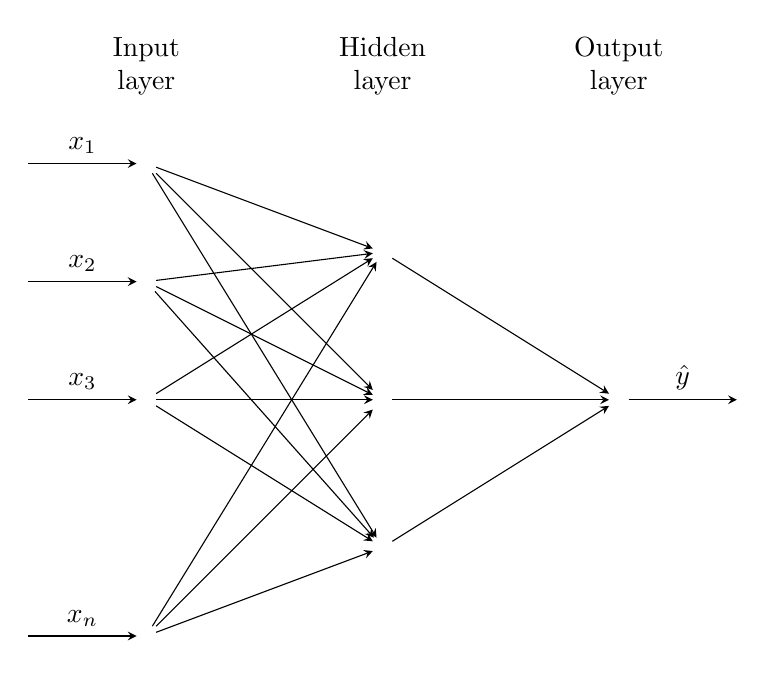
\begin{tikzpicture}[x=1.5cm, y=1.5cm, >=stealth]

\foreach \m/\l [count=\y] in {1,2,3,missing,4}
  \node [every neuron/.try, neuron \m/.try] (input-\m) at (0,2.5-\y) {};

\foreach \m [count=\y] in {1,2,3}
  \node [every neuron/.try, neuron \m/.try ] (hidden-\m) at (2,2-\y*1.25) {};

\foreach \m [count=\y] in {1}
  \node [every neuron/.try, neuron \m/.try ] (output-\y) at (4,0.5-\y) {};

\foreach \l [count=\i] in {1,2,3,n}
  \draw [<-] (input-\i) -- ++(-1,0)
    node [above, midway] {$x_\l$};

\foreach \l [count=\i] in {1}
  \draw [->] (output-\i) -- ++(1,0)
    node [above, midway] {$\hat{y}$};

\foreach \i in {1,...,4}
  \foreach \j in {1,...,3}
    \draw [->] (input-\i) -- (hidden-\j);

\foreach \i in {1,...,3}
  \foreach \j in {1,...,1}
    \draw [->] (hidden-\i) -- (output-\j);

\foreach \l [count=\x from 0] in {Input, Hidden, Output}
  \node [align=center, above] at (\x*2,2) {\l \\ layer};

\end{tikzpicture}
\caption{Illustration of a MLP model.} \label{fig:mlp}
\end{figure}

\section{Exploding and Vanishing Gradients} \label{sec:gradients}
Having the sequential architecture described in section \ref{sec:bbann} MLPs faces an additional implementation challenge that is not common in traditional machine learning, the difficulty of training. 
The typical training process for the machine learning algorithm is at a very high level is a standard procedure.  
The first step is to feeding input data to model and produce an output, then based on desired output for the input loss value can be calculated.
Loss value is a calculation of how much the output is further away from the desired output. 
Using this loss value we can approximate weight updates with the help of the optimization algorithm until the model weights converge.
Even though the training process is also the same for the MLPs there is more complexity involved in MLPs giving that instead of dealing with one model we have layers of neurons chained together that each has its own weights. 
For those reasons training MLPs was a challenge until the influential \emph{backpropagation} paper~\cite{backprop} is published. In this paper efficient technique of calculating the gradients using forward and backwards passes demonstrated.
Utilizing the chain rule of calculus, the backpropagation algorithm was able to calculate the update for each weight in every neuron.

Notwithstanding help of the backpropagation algorithm, as the need for training deeper networks increased, the difficulty of training such networks remained a problem.
Part of the problem was, as the gradients get smaller and smaller as the gradient flowed down to lower layers (layers close to the input layer) of the network. 
When the gradient updates get close to very small values some of the lower layer weights do not updated enough and consequently not converging model to appropriate representation.
This phenomenon is usually referred to as \emph{vanishing gradients} problem.
Similarly, some network such as recurrent neural networks can have an opposite problem that resulting in gradients getting larger and larger which pushes weights to be a very large number. 
Similarly, this phenomenon referred to as the \emph{exploding gradients} problem.
Later on, this unstable gradient flow problems are shown to be the combination of choice for weight initialization and the characteristic of the activation functions that widely used~\cite{vanishgrads}.
Previously, activation function often get used was the sigmoid (also known as logistic function) \(\sigma(x) = \frac{1}{1 + e^{-x}}\) and the hyperbolic tangent function (\(tanh(x) = 2\sigma(2x) -1\)) have a flatten tails where \textbf{\textit{x}} get very large or very small. 
Giving that the chain rule states that the derivative of a variable is equal to the product of the partial derivatives of the composite function with respect to output, neurons that produce an output very large and very small will not likely to be updated. 
For example lets suppose \(\hat{y} = \sigma(z(w, b))\) and \(z(w, b) = wx + b\). Then chain rule states that

\begin{equation} \label{eq:chain}
  \frac{\partial{\hat{y}}}{\partial{w}} = \frac{\partial{\hat{y}}}{\partial{\sigma}}  \frac{\partial{\sigma}}{\partial{w}}
\end{equation}

It is clear that the gradient update of \textbf{\textit{w}} is predicated on the gradient of the $\sigma$ is not being zero.
While the sigmoid and hyperbolic tangent functions derivatives get close to zero when the functions are on the saturating region. 

\begin{figure}[H]
  \centering
  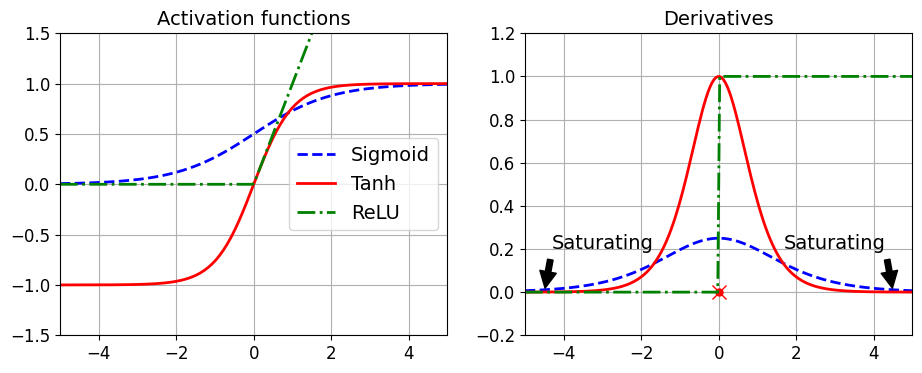
\includegraphics[width=\textwidth]{img/activation_functions_plot.png}
  \caption{Saturation points in activation functions.}
  \label{fig:saturate}
\end{figure}

Due to these properties, \emph{Rectified Linear Unit} (ReLU) activation function emerges as a good alternative to train deeper neural networks.
ReLU behaves like a linear function for the non-negative values ($f(x) = max(0, x)$) and outputs zero for the negative input values.
With that characteristic gradient of the ReLU will be either zero for the input values less than or equal to zero and one for any other values.
Because of consistent properties of the non-saturating functions, it is always better to use such activation functions for hidden layers to ensure the gradient flow is faster and Network will converge faster as a result.

\section{Optimization} \label{sec:optimization}
Most machine learning algorithms utilize some sort of optimization. 
The main objective of the optimization algorithms is to find the maximum or the minimum point for the function in hand with respect to one or more variable. 
For the machine learning domain, we would like to optimize the loss function (also known as a cost function) to the global minimum for having a model that is most representative of the data.
The task of searching minimum or maximum can be used interchangeably as finding the minimum point of the function $f$ may also be found by getting maximum of the inverse function of the same function ($f^{-1}$).
In essence, the process is achieved by taking derivative of the function which will give us a slope for the given point, the moving opposite to the slope with the small increments until we reach to the minimum point where the gradient is zero.
The process also known as \emph{gradient descent}.
Gradient descent used in machine learning field for a long time, however depending on the complexity of the function space this process could take a significantly long time. 
For mitigating this problem new set of algorithms called \emph{momentum optimizers} created.
The difference between these algorithms and gradient descent is simply, gradient descent will take small consistent steps regularly throughout the optimization process. 
How these momentum-based algorithms works are they generally pay attention to the previous gradients and accelerate the updates based on gradients and the slope at the point of the gradient. 
This will help the optimization to converge to global minimum faster when there is a lot of plateau areas in the function surface.
Later on, momentum algorithms expanded to include taking the steepest dimension of the gradient to point updates more toward to the global minimum, a new family of optimizers named as \emph{adaptive} optimizers. 
Most well know algorithms of this category is AdaGrad~\cite{adagrad}, RMSProp~\cite{rmsprop}, Adam~\cite{adam} and Nadam~\cite{nadam}.
Despite the fact, these adaptive optimizers usually converge to good solutions faster research by Ashia C. Wilson et al~\cite{optimize-ashia}. showed that in some cases these optimizers can lead to poor generalization result depending on the dataset.
It might be good practice to try adaptive and momentum-based optimizers in the training job to observe their effect in generalization.


\section{Regularization and Over-fitting} \label{sec:regularization}
Generally, the fundamental challenge in machine learning is that our model should perform well on previously unseen data points which is also referred to as generalization.
If the scope of the model is sufficiently large (model with a large number of parameters) optimization techniques described previously could enable the model to capture noise that specific to training records. 
In other words \emph{overfitting} is where the model will focus on individual nuances of data records instead of focusing on general pattern overall.
However, there are numerous regularization techniques available to mitigate the overfitting in ANNs.
Just like traditional machine learning \textit{l} regularization (norm) can be applied to the artificial neural networks.
In general form $l_p$ norm is given by

\begin{equation}
  \left\lVert x \right\rVert_p = \left(\sum_i \left\lvert x_i \right\rvert^p \right) ^{\frac{1}{p}}
\end{equation}

for vector \textbf{\textit{x}} and $p \in \mathbb{R}$, $p \geq 1$.

Most frequently used $l$ norms are $l_1$ and $l_2$ regularization.
The $l_1$ norm usually used when the difference between elements are important. 
This regularization seldom referred to as \emph{Manhatten distance} in the literature.
Similarly, another norm get used often is $l_2$ norm, also known as \emph{Euclidean distance}, is the geometric distance between points and could be calculated simply as $x^Tx$

In addition to $l_p$ norms \emph{dropout}~\cite{dropout} emerges as a popular regularization technique specific to the ANNs.
Dropout is a process of removing a fraction of the units from a neural network layer by setting the weight of the unit to zero during training.
This technique reduces the reliance of each unit for the prediction.
In each training iteration fraction of the neurons dropped randomly so the remain neurons are forced to train in the absence of the neurons picked.
Although dropout has proven to improve generalization in many machine learning tasks, due to its unstable nature time it takes for the network to converge usually increases.



\section{Convolutional Networks} \label{sec:convnets}
In the proposal of this project, I used the definition from Deep Learning book~\cite{deeplearningbook} for the definition of Convolutional Neural Networks (CNNs) that I believe summarize the concept very well. 
To quote that definition again CNNs are:
\begin{quote}
  "Convolutional networks are simply neural networks that use convolution in place of general matrix multiplication in at least one of their layers."
\end{quote}

In CNN's neurons replaced by units usually called kernel or filter.
These units are rectangular matrix span over the layers of the input data. 
The way this unit calculates its output by positioning each kernel item to pixels on the image and calculate the element-wise multiplication between them. 
The kernel then slides over the rest of the image until all image covered. 
The area that processed by the image is called \emph{receptive field} and operating this way by calculating each area in image CNNs are able to capture information about the locality of the image as opposed to flattening.
The output of the operation depends on the design of the convolution operation.
There are two main concept defines the operation, one is stride or how many pixels the kernel will be moved to complete the operation, and the size of the padding.
Padding is zero value pixels that get placed around the image to centralize the items at the edge of the image in kernels.

The output of the convolutional network can be calculated easily to ensure no bug is introduced to the model during implementation.
Given the volume size of the input image (\textbf{\textit{I}}), kernel size of CNN (\textbf{\textit{K}}), stride which is applied (\textbf{\textit{S}}), and the amount of zero padding applied is (\textbf{\textit{P}}). We can calculate the output as:

\begin{equation}
  output = \frac{(I - K + 2P)}{S} + 1  
\end{equation}

The generally accepted way of padding in convolution operations are, the SAME and the VALID padding.
SAME padding is using zero paddings around the image to output \emph{same} size output from the convolution when chosen a stride is one.
VALID padding, however, is a practice of not applying any zero paddings and only uses \emph{valid} pixels from the image.

Conventionally, convolutional layers are used together with the pooling layer.
The main contribution of the pooling layer is to under-sample the output data.
Doing so they will reduce the memory usage and the computational complexity of the network.
Additionally reducing the size of the output will reduce the chance of overfitting.
Most frequently used versions of the pooling layer are max pooling and average pooling.
Regardless of the operation pooling layer works by choosing the pool size and applying the desired operation to that field in the input.
For example, if it is a max-pooling layer, the maximum pixel value in the polling size is passed on to the next layer.


\section{Software Challenges Specific to 
Machine Learning Systems} \label{sec:engchallenge}
It is clear from some of the problems mentioned earlier, training deep neural networks is a difficult task. 
One particular reason for difficulty when applying ANNs to new fields is identifying the problem when getting bad scores from the model. 
Because unlike tradition software development it is difficult to know whether there is a bug in the implementation of the software or the model itself is not suitable to represent the underlying data distribution.
For overcoming this challenge I am employing a diagnosis and debugging check list that will help identify and eliminate any bugs that can occur in the implementation phase.
Where applicable checklist points are:

\begin{itemize}
  \item Overfit to sample data to ensure no optimization mistakes made.
  \item Monitor training loss during training and make sure it is declining throughout the training.
  \item Check the input and output shapes are correct.
  \item Make minor changes to models and only add addition changes after ensuring there is no bug in the system.
\end{itemize}

Another challenge is the computationally expensive nature of the training.
Due to the iterative nature of the machine learning, it is vital that the experimentation for the task will run sufficiently quick that the improvement for the model can be identified quickly and progressed to further stages. 
However, standard ANNs usually have millions of parameters that need to be updated while training with hundreds of thousands if not millions of training examples to train on. 
Considering the average training process will need multiple passes on the entire dataset, the need for high computation power becomes evident.
That's why most training is done with the help of hardware accelerators such as GPUs or TPUs.
Choice of computation environment for this project luckily includes such hardware accelerators but these special hardwares must be detected and enabled so the calculation can take advantage of the compute power.
To enable the hardware related capabilities and to reduce training management overhead I have written a wrapper module in the custom code library.
Some of the other features that made possible with this module are:

\begin{itemize}
  \item Ability to detect and set the hardware accelerators.
  \item Choosing training strategy suitable for the hardware accelerator.
  \item Logging performance metrics persistently.
  \item Saving model persistently in case of computing failure and continue where the training left previously.
  \item Extract final model with runtime data.
\end{itemize}
 
Possibly one of the most important features of the helper library is providing resilient training. 
Some large models take hours or days to train and my choice of computation environment allows only twelve-hour training before terminating. 
Not to mention virtual machines power that environment might disconnect or terminate much earlier. 
In the case of such an event, if all the previous training is lost, time spent on training will be wasted. 
If similar events happen many more times it could even risk not completing all the experimentations on time for this project deadline. 
To eliminate that risk, I have implemented a process that will save model weight to storage outside the compute environment regularly. 
If such failure happens, the module will pick up the last saved weights and continue to training where it left of previously.
In addition to starting the training with the previous model, by using naming conventions, the module can initialize the epoch number for the training accordingly and allow accurate comparison between other models. 
In other words, if the first training attempt is failed in epoch number 23 restarting training will start with the epoch number 23.

\section{Literature Review}
The aim of this project is building an automated CI/CD machine learning pipeline for classification of X-ray images.
Or to summarize Mlops applied to medical imaging.
Therefore it is practical to split the relevant works reviewed for this project to two distinct categories, mlops and computer vision in medical imaging.



\clearpage